%
\section{Statische Analyse}
Zur statischen Analyse von C\# Programmen stehen eine Reihen an Werkzeugen zur Verfügung. Einerseits gibt es in die Entwicklungsumgebung integrierte Werkzeuge wie \emph{NDepend}, \emph{ReSharper} und das von Visual Studio bereitgestellt Tool, andererseits eigenständige Programme wie \emph{Gendarme} und \emph{SourceMonitor}.

\subsection{NDepend}
\emph{NDepend} führt statischen Analysen von Projekten durch, erstellt dabei Softwarelandkarten, Codemetriken und überprüft ob Quelltextregel eingehalten werden.~\cite{ndepend} Auf der \enquote{Dashboard} genannten Übersicht erstellt NDepend eine Zusammenfassung aller Analysen. 

\subsubsection{Quelltextregel}
NDepend ermittelt in C\# Essentials insgesamt 37 verletzte Regeln, dabei finden 150 Regeln Anwendung. An dieser Stelle soll nur auf die als kritisch markierten Regeln eingegangen werden. 3 kritische Regelverletzungen ermittelt NDepend: Methods too complex (2), Potenially dead Methods (6), Potentially dead Types (6). Weitere verletzte Regeln sind in erster Linie nicht eingehaltene Namenskonventionen, Sichtbarkeiten und Design Schwächen. Kritische Stellen werden im folgenden genauer analysiert, um potentielle Fehler zu finden.

\paragraph{Methods too complex}

\paragraph{Potentially dead Methods} In C\# Essentials findet NDepend sechs mögliche Stellen, an denen Quelltext nicht ausgeführt wird. In Abbildung~\ref{fig:dead-methods} sieht man zwei der gefundenen Stellen. Bei allen handelt es sich um nicht aufgerufenen Konstruktoren. 

\begin{figure}[ht]
\centering
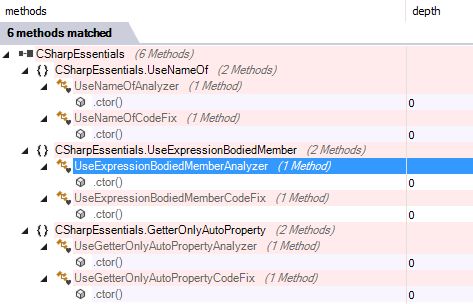
\includegraphics[width=0.8\textwidth]{images/dead-methods.png}
\caption{Potentially dead Methods}
\vspace{0.1cm}
Von NDepend gefundener wahrscheinlich nicht aufgerufener Quelltext
\label{fig:dead-methods}
\end{figure}

\subsubsection{Quelltextmetriken}
Mit Hilfe des \enquote{Code Metrics View} visualisiert \emph{NDepend} Quelltextmetriken in

\paragraph{Interpretation der Quelltextmetriken}
Mit dem \enquote{Code Metrics View} Werkzeug

\subsection{ReSharper}
Mit \emph{ReSharper} bietet JetBrains ein Werkzeug zur statischen Analyse für Visual Studio an.~\cite{resharper} 

\subsection{Visual Studio Tools}
Visual Studio analysiert Code, erstellt dabei Quelltextmetriken und kann zum Beispiel Code-Clone identifizieren.

\subsubsection{Quelltextmetriken}

\subsubsection{Code-Clone}


\subsection{Gendarme}
Gendarme analysiert Programme und Bibliotheken, welche in den verschiedenen .NET Sprachen geschrieben wurden. Dafür benötigt Gendarme eine kompilierte Assembly, weil es nicht den C\# statisch analysiert, sondern ein daraus erzeugte Spracheformat: Das ECMA CIL~\footnote{European Computer Manufacturers Association Common Language Infrastructure} Format.~\cite{ecma} Die CIL wird mit Hilfe von der Bibliothek Cecil analysiert.~\cite{cecil} Gendarme generiert auf Basis dieser Analyse Berichte. Sie können als HTML-Datei exportiert werden.

\paragraph{ECMA CIL}

\subsubsection{Fehler}

\subsubsection{Sicherheit}


\subsection{SourceMonitor}
Der Fokus von \emph{Source Monitor} liegt auf der Analyse von Quelltextmetriken. Es bietet die Möglichkeit einzelne 

\subsubsection{Kiviat-Chart}
